
\begin{center}
\Huge
Linjens ligning og parameterfremstilling
\end{center}


\section*{Linjens ligning}
\stepcounter{section}

I analytisk geometri ønsker vi at beskrive geometriske objekter ved brug af ligninger og koordinatsystemer i stedet for at analysere geometriske objekter ved hjælp af lineal, passer og lignende. Vi vil eksempelvis se på ligninger for linjer og cirkler - desuden skal vi se, hvordan vi kan \textit{parametrisere} en linje. Vi lægger ud med at udlede linjens ligning.

Vi får brug for begrebet \textit{normalvektor}, der blot er en vektor $\vv{n}$, der står ortogonalt på et objekt. Vi kan altså både have normalvektorer til fx linjer og andre vektorer. 
Vi lader $l$ være en vilkårlig linje og vi lader $P(x_0,y_0)$ være et punkt på denne linje. Vi kan danne en forbindelsesvektor $\vv{v}$ fra $(x_0,y_0)$ til ethvert andet punkt $(x,y)$ på $l$ ved
\begin{align}\label{eq:eq1}
\vv{v} = \begin{pmatrix}
x-x_0\\y-y_0
\end{pmatrix}.
\end{align}
For en normalvektor $\vv{n}$ til $l$ givet ved
\begin{align*}
	\vv{n} = 
	\begin{pmatrix}
		a\\b
	\end{pmatrix}
\end{align*}
vil det gælde, at prikproduktet mellem $\vv{v}$ og $\vv{n}$ er lig 0, altså at $\vv{v}\cdot \vv{n} = 0$. Mere specifikt har vi, at 
\begin{align*}
	\begin{pmatrix}
		x-x_0\\ y-y_0
	\end{pmatrix} \cdot 
	\begin{pmatrix}
		a \\ b
	\end{pmatrix} = 0,
\end{align*}
hvilket medfører, at 
\begin{align*}
a(x-x_0) + b(y-y_0) = 0.
\end{align*}
Linjen $l$ samt vektorerne $\vv{v}$ og $\vv{n}$ kan ses af Fig. \ref{fig:linjeligning}.
\begin{figure}[H]
	\centering
	\begin{tikzpicture}
		\begin{axis}[axis lines = middle,
		xmin = -1, 
		ymin = -1,
		ticks = none		
		]
			\addplot[color = teal, thick] {0.6*x+1};
			\draw[-{Stealth[scale=1.5]}, thick] (axis cs:1,1.6) -- (axis cs:3,2.8);
			\node[color = teal] at (axis cs:4.7,3.5) {$l$};
			\node at (axis cs:2,2.4) {$\vv{v}$};
			\draw[-{Stealth[scale = 1.5]},thick] (axis cs:1,1.6) -- (axis cs:2.2,-0.4);
			\node at (axis cs:1.7,0.9) {$\vv{n}$};
			\node[circle, fill = olive, inner sep = 0pt, minimum size = 5pt] at (axis cs: 1,1.6) {};
			\node[color = olive] at (axis cs: 0.7,1.9) {$(x_0,y_0)$};
			\node[circle, fill = olive, inner sep = 0pt, minimum size = 5pt] at (axis cs:3,2.8) {};
			\node[color = olive] at (axis cs: 2.8,3.1) {$(x,y)$};
			\draw[dashed] (axis cs:1.22,1.28) -- (axis cs:1.54,1.48);
			\draw[dashed] (axis cs:1.35,1.81) -- (axis cs:1.54,1.48);
		\end{axis}
	\end{tikzpicture}
	\caption{Retningsvektor og normalvektor til linjen $l$.}
	\label{fig:linjeligning}
\end{figure}
Vi kan nu konkludere med en sætning.
\begin{setn}[Linjens ligning]
Lad $l$ være en linje med en normalvektor $\vv{n}$ givet ved
\begin{align*}
	\vv{n} = 
	\begin{pmatrix}
		a\\b
	\end{pmatrix},
\end{align*} og lad $P(x_0,y_0)$ være  et punkt på linjen. Så opfylder ethvert punkt $(x,y)$, der ligger på linjen $l$, at 
\begin{align}\label{eq:linjensligning}
a(x-x_0) + b(y-y_0) = 0.
\end{align}
Vi kalder ligningen \eqref{eq:linjensligning} for \textit{linjens ligning}. Mere præcist er \eqref{eq:linjensligning} ligningen for linjen $l$.
\end{setn}
\begin{exa}
På linjen $l$ kender vi punktet $P(-1,3)$ og normalvektoren $\vv{n} = \begin{pmatrix}
2 \\ 4
\end{pmatrix}$. Ligningen for $l$ er derfor givet
\begin{align*}
2(x+1) + 4(y-3) = 0.
\end{align*}
\end{exa}

\begin{exa}
En linje $l$ har ligningen 
\begin{align}\label{eq:ex2}
	3(x+1) + 4(y-1) = 0.
\end{align}
Vi vil undersøge, om punkterne $(3,-2)$ og $(1,0)$ ligger på $l$. Vi indsætter derfor punkterne i \eqref{eq:ex2} og regner efter. Det første punkt giver
\begin{align*}
3(x+1) + 4(y-1) = 0 \ &\Leftrightarrow \  3(3+1) + 4(-2-1) = 0 \\
& \Leftrightarrow \ 3\cdot 4+4\cdot(-3) = 0\\
% \Leftrightarrow \ 0 = 0,
\end{align*}
og derfor ligger punktet $(3,-2)$ på $l$. Tilsvarende for det andet punkt fås
\begin{align*}
3(1+1) + 4(0-1) = 0 \  \Leftrightarrow \ 2 = 0, 
\end{align*}
hvilket tydelige er et falsk udsagn. Derfor ligger punktet $(1,0)$ ikke på linjen $l$. 
\end{exa}
\begin{exa}
	En linje $j$ er givet ved ligningen
	\begin{align*}
		j:\ 2(x-3) + 5(y-2) = 0,
	\end{align*}
	og vi ønsker at omskrive den til formen
	\begin{align*}
		y = ax + b
	\end{align*}
	for to tal $a$ og $b$. Vi hæver parenteserne og omskriver
	\begin{align*}
		2(x-3) + 5(y-2) = 0 \ &\Leftrightarrow \ 2x - 6 + 5y - 10 = 0\\
		&\Leftrightarrow	\ 2x + 5y - 16 = 0 \\
		&\Leftrightarrow \ 5y = -2x + 16 \\
		&\Leftrightarrow \ y = \frac{-2}{5}x + \frac{16}{5},
	\end{align*}
	og ligningen er omskrevet, så vi kan se hældningen og skæringen med andenaksen for linjen. 
\end{exa}



\section*{Linjens Parameterfremstilling}
\stepcounter{section}

I stedet for at repræsentere en linje ved hjælp af et punkt $P(x_0,y_0)$ og en normalvektor $\vv{n}$, så kan vi repræsentere linjen ved hjælp af et punkt $P(x_0,y_0)$ og en \textit{retningsvektor} $\vv{r}$ givet ved 
\begin{align*}
	\vv{r} = 	
	\begin{pmatrix}
 		r_1 \\ r_2
	\end{pmatrix}.
\end{align*}

så må punktet $(x,y)$, der opfylder, at
\begin{align*}
\begin{pmatrix}
x \\ y
\end{pmatrix}
= \begin{pmatrix}
x_0 \\ y_0
\end{pmatrix} + \begin{pmatrix}
r_1 \\ r_2
\end{pmatrix}
\end{align*}
ligge på $l$. Men for alle tal $t$ ved vi, at alle vektorer $t\vv{r}$ er parallelle med $\vv{r}.$ Derfor må der desuden gælde, at alle punkter $(x,y)$, der opfylder, at 
\begin{align*}
\begin{pmatrix}
x \\ y
\end{pmatrix}
=
\begin{pmatrix}
x_0 \\ y_0
\end{pmatrix} 
+
t
\begin{pmatrix}
r_1 \\ r_2
\end{pmatrix}
 \end{align*}
må være præcist de punkter, der ligger på linjen $l$. Dette kan ses af Figur \ref{fig:linjeligning}
\begin{figure}[H]
	\centering
	\begin{tikzpicture}
		\begin{axis}[axis lines = middle,
		xmin = -1, 
		ymin = -1,
		ticks = none		
		]
			\addplot[color = teal, thick] {0.6*x+1};
			
			\draw[-{Stealth[scale=1.5]}, thick, olive] (axis cs:1,1.6) -- (axis cs:4,3.4);
			\draw[-{Stealth[scale=1.5]}, thick] (axis cs:1,1.6) -- (axis cs:3,2.8);
			\node[color = teal] at (axis cs:4.7,3.5) {$l$};
			\node at (axis cs:2,2.4) {$\vv{r}$};
			
			
			\node[circle, fill = olive, inner sep = 0pt, minimum size = 5pt] at (axis cs: 1,1.6) {};
			\node[color = olive] at (axis cs: 0.7,1.9) {$(x_0,y_0)$};
			\node[circle, fill = olive, inner sep = 0pt, minimum size = 5pt] at (axis cs:4,3.4) {};
			\node[color = olive] at (axis cs: 3.8,3.7) {$(x,y)$};
			
			
		\end{axis}
	\end{tikzpicture}
	\caption{Retningsvektor til linjen $l$.}
	\label{fig:linjeligning}
\end{figure}
\newpage
Vi kan nu igen konkludere med en sætning.
\begin{setn}[Linjens parameterfremstilling]
For en linje $l$ gælder der, at alle punkter $(x,y)$, der ligger på $l$ opfylder, at
\begin{align*}
\begin{pmatrix}
x \\ y
\end{pmatrix}
=
\begin{pmatrix}
x_0 \\ y_0
\end{pmatrix} 
+
t
\begin{pmatrix}
r_1 \\ r_2
\end{pmatrix},
\end{align*} 
hvor $P(x_0,y_0)$, $\vv{r} = \begin{pmatrix}
r_1 \\ r_2
\end{pmatrix}$
er en retningsvektor for linjen og $t$ er et vilkårligt tal. Vi kalder dette for \textit{parameterfremstillingen for l}.
\end{setn}
\begin{defn}[Tværvektor]
	Lad $\vv{v}$ være givet ved
	\begin{align*}
		\vv{v} = 
		\begin{pmatrix}
			a \\ b
		\end{pmatrix}.
	\end{align*}
	Så defineres \textit{tværvektoren} $\widehat{\vv{v}}$ til $\vv{v}$ som 
	\begin{align*}
		\widehat{\vv{v}} = 
		\begin{pmatrix}
			-b \\ a
		\end{pmatrix}.
	\end{align*}
\end{defn}
Det er ikke svært at overbevise sig selv om at en vektor $\vv{v}$ og dens tværvektor $\widehat{\vv{v}}$ er orthogonale. Tjekker vi efter, får vi, at 
\begin{align*}
	\vv{v} \cdot \widehat{\vv{v}} = 
	\begin{pmatrix}
		a \\ b
	\end{pmatrix} \cdot
	\begin{pmatrix}
		-b \\ a
	\end{pmatrix} = 
	a\cdot b - b\cdot a = 0. 
\end{align*}
\begin{exa}
Har vi et punkt $P = (-1,3)$ og en retningsvektor $\vv{r} = \begin{pmatrix}
5 \\ 1
\end{pmatrix}$ kan vi bestemme parameterfremstillingen for linjen $l$, der går gennem $P$ og har retningsvektor $\vv{r}$:
\begin{align*}
\begin{pmatrix}
x \\ y
\end{pmatrix}
= 
\begin{pmatrix}
-1 \\ 3
\end{pmatrix} +  
t
\begin{pmatrix}
5 \\ 1
\end{pmatrix}.
\end{align*}
Da $\begin{pmatrix}
-1 \\ 5
\end{pmatrix}$
er orthogonal til $\vv{r}$ vil denne vektor være en normalvektor til $l$. Vi kan derfor også repræsentere $l$ ved ligningen
\begin{align*}
-1(x+1) + 5(y-3) = 0.
\end{align*}
\end{exa}

\begin{exa}
	En linje $l$ har parameterfremstillingen
	\begin{align*}
		l: \  \begin{pmatrix} x \\ y \end{pmatrix} = 
		\begin{pmatrix} 1 \\ -2 \end{pmatrix} + t
		\begin{pmatrix}
			4\\2
		\end{pmatrix}.
	\end{align*}
	Vi skal afgøre, om punkterne $(1,1)$ og $(5,0)$ ligger på $l$. Vi indsætter første punkt i 
	parameterfremstillingen.
	\begin{align*}
		\begin{pmatrix}
			1 \\ 1
		\end{pmatrix} =
		\begin{pmatrix}
			1 \\ -2
		\end{pmatrix} + t
		\begin{pmatrix}
			4 \\ 2
		\end{pmatrix}.
	\end{align*}
	I første linje har vi ligningen
	\begin{align*}
		1 = 1 + t\cdot 4,
	\end{align*}
	så $t = 0$. Det indsættes i den nederste ligning:
	\begin{align*}
		1 = -2 + 0\cdot  2 = -2,
	\end{align*}
	hvilket ikke er korrekt. Derfor ligger punktet $(1,1)$ ikke på linjen $l$. 
	Tilsvarende indsættes punktet $(5,0)$, og vi får
	\begin{align*}
		\begin{pmatrix}
			5 \\ 0
		\end{pmatrix} = 
		\begin{pmatrix}
			1 \\ -2
		\end{pmatrix} + t
		\begin{pmatrix}
			4 \\ 2
		\end{pmatrix}.
	\end{align*}
	Første ligning lyder så
	\begin{align*}
		5 = 1 + t\cdot 4,
	\end{align*}
	så $t = 1$. Dette indsættes i anden ligning:
	\begin{align*}
		0 = -2 + 1\cdot 2 = 0,
	\end{align*}
	hvilket er sandt, så punktet $(5,0)$ ligger på linjen $l$. 
\end{exa}



\subsection*{Opgave 1}
\begin{enumerate}[label=\roman*)]
\item Afgør, om punkterne $(0,2)$ og $(-2,3)$ ligger på linjen med ligningen
\begin{align*}
	(x-2) + 2(y-1) = 0.
\end{align*}
\item Afgør, om punkterne $(-4,-1)$ og $(-3,6)$ ligger på linjen med ligningen 
\begin{align*}
	5(x+5) - 2(y-1) = 0.
\end{align*}
\end{enumerate}

\subsection*{Opgave 2}
Bestem linjens ligning for følgende punkter $P(x_0,y_0)$ og normalvektorer $$\vv{n} = \begin{pmatrix}
a \\ b
\end{pmatrix}.$$
\begin{align*}
&1) \ P(1,1), \ \vv{n} = \begin{pmatrix}
-2 \\ 3
\end{pmatrix}.   &&2) \ P(-5,-3), \ \vv{n} = \begin{pmatrix}
2 \\ 7
\end{pmatrix}.    \\
&3) \ P\left(\frac{-2}{5},13\right), \ \vv{n} = \begin{pmatrix}
-10 \\ 20
\end{pmatrix}.   &&4) \ P(\sqrt{2},\sqrt{3}), \ \vv{n} = \begin{pmatrix}
\frac{1}{5} \\ \frac{7}{10}
\end{pmatrix}.   \\
&5) \ P(0,0), \ \vv{n} = \begin{pmatrix}
1 \\ 1
\end{pmatrix}.   &&6) \ P(-100,5), \ \vv{n} = \begin{pmatrix}
-\frac{\sqrt{2}}{2} \\ -9
\end{pmatrix}.   \\
\end{align*}

\subsection*{Opgave 3}
Vi har tidligere set linjer repræsenteret på formen $y = ax+b$, og har vi en ligning på formen $a(x-x_0) + b(y-y_0) = 0$, så kan denne omskrives til formen\\ $y = ax+b$ (bemærk, at konstanterne $a$ og $b$ uheldigvis ikke her har samme betydning). Omskriv følgende ligninger fra formen $a(x-x_0) + b(y-y_0) = 0$ til formen $y=ax+b$. Tjek at dit resultatet er korrekt ved at tegne begge linjer i eksempelvis Geogebra. 

\begin{align*}
&1) \ 2(x+2) + 3(y+3) = 0 &&2) \ -7(x-1) + 6(y-1) = 0\\
&3) \ (x+10) + (y-9) = 0 &&4) \ 5(x-5) + 4(y-0.5) = 0\\
\end{align*}

\subsection*{Opgave 4}
I følgende koordinatsystemer er tegnet en linje $l$ samt en normalvektor til linjen. Brug koordinatsystemerne til at bestemme linjens ligning for hver af linjerne.
\begin{center}
\resizebox{0.45\textwidth}{0.45\textwidth}{
\begin{tikzpicture}
	\begin{axis}[axis lines = middle, grid, xmin = -0.5, xmax = 5.5, ymin = -0.5, ymax = 5.5]
		\addplot[color = teal, thick] {-0.5*x+3};
		\draw[-{Stealth[scale = 1.5]}, color = olive, thick] (axis cs:2,2) -- (axis cs: 3, 4);
	\end{axis}
\end{tikzpicture}
}
\resizebox{0.45\textwidth}{0.45\textwidth}{
\begin{tikzpicture}
	\begin{axis}[axis lines = middle, grid, xmin = -3.5, xmax = 3.5, ymin = -1.5,ymax = 5.5]
		\addplot[color = teal, thick] {2*x+6};
		\draw[-{Stealth[scale = 1.5]}, color = olive, thick] (axis cs:-1,4) -- (axis cs: 3, 2);
	\end{axis}
\end{tikzpicture}
}
\end{center}
\begin{center}
\resizebox{0.45\textwidth}{0.45\textwidth}{
\begin{tikzpicture}
	\begin{axis}[axis lines = middle, grid, xmin = -1.5, xmax = 3.5, ymin = -1.5,ymax = 3.5]
		\addplot[color = teal, thick] {-x+1};
		\draw[-{Stealth[scale = 1.5]}, color = olive, thick] (axis cs:1,0) -- (axis cs: 2, 1);
	\end{axis}
\end{tikzpicture}
}
\resizebox{0.45\textwidth}{0.45\textwidth}{
\begin{tikzpicture}
	\begin{axis}[axis lines = middle, grid,xmin = -1.5, xmax = 3.5, ymin = -1.5,ymax = 3.5]
		\addplot[color = teal, thick] {2};
		\draw[-{Stealth[scale = 1.5]}, color = olive, thick] (axis cs:2,2) -- (axis cs: 2, -1);
	\end{axis}
\end{tikzpicture}
}
\end{center}
 
\subsection*{Opgave 5}
Følgende linjer er repræsenteret på formen $y = ax + b$. Tegn dem i GeoGebra og bestem så et punkt $P(x_0,y_0)$ på linjen samt en normalvektor $\vv{n}$ til linjerne. Brug punktet $P$ og normalvektoren $\vv{n}$ til at omskrive ligningen for linjen fra formen $y = ax+b$ til formen $a(x-x_0) + b(y-y_0) = 0$. 
\begin{align*}
	&1) \ y = 2x+1 &&2) \ y = -\frac{1}{4}x-2\\
	&3) \ y = x-7 &&4) \ y = 5x+0.6\\
	&5) \ y = 12x-13 &&6) \ y = -4x\\
\end{align*}


\subsection*{Opgave 6}
Bestem en parameterfremstilling for følgende linjer, der har retningsvektorer $$\vv{r} = \begin{pmatrix}
r_1 \\ r_2
\end{pmatrix}$$ og hvor punkterne $P(x_0,y_0)$ ligger på linjen.
\begin{align*}
&1) \ P(1,1), \ \vv{r} = \begin{pmatrix}
-2 \\ 3
\end{pmatrix}.   &&2) \ P(-5,-3), \ \vv{r} = \begin{pmatrix}
2 \\ 7
\end{pmatrix}.    \\
&3) \ P\left(\frac{-2}{5},13\right), \ \vv{r} = \begin{pmatrix}
-10 \\ 20
\end{pmatrix}.   &&4) \ P(\sqrt{2},\sqrt{3}), \ \vv{r} = \begin{pmatrix}
\frac{1}{5} \\ \frac{7}{10}
\end{pmatrix}.   \\
&5) \ P(0,0), \ \vv{r} = \begin{pmatrix}
1 \\ 1
\end{pmatrix}.   &&6) \ P(-100,5), \ \vv{r} = \begin{pmatrix}
-\frac{\sqrt{2}}{2} \\ -9
\end{pmatrix}.   \\
\end{align*}

\subsection*{Opgave 7}
\begin{enumerate}[label=\roman*)]
	\item En linje $l$ har parameterfremstillingen
	\begin{align*}
		l: \ 
		\begin{pmatrix}
			x \\ y
		\end{pmatrix}=
		\begin{pmatrix}
			3 \\5
		\end{pmatrix} + t
		\begin{pmatrix}
			-1 \\ 1
		\end{pmatrix}.
	\end{align*}
	Afgør, om punkterne $(3,-2)$ og $(2,2)$ ligger på $l$. 
	\item En linje $l$ har parameterfremstillingen
	\begin{align*}
		l: \ 
		\begin{pmatrix}
			x \\ y
		\end{pmatrix}=
		\begin{pmatrix}
			-2 \\2
		\end{pmatrix} + t
		\begin{pmatrix}
			6 \\ -7  
		\end{pmatrix}.
	\end{align*}
	Afgør, om punkterne $(0,0)$ og $(16,23)$ ligger på $l$. 
\end{enumerate}

\subsection*{Opgave 8}

\begin{enumerate}[label=\roman*)]
\item Bestem en parameterfremstilling for linjen $l$ givet ved ligningen 
\begin{align*}
2(x-2) + 3(y+1) = 0.
\end{align*}
\item Bestem en parameterfremstilling for linjen $l$ givet ved ligningen 
\begin{align*}
-10(x-10) + 10(y+10) = 0.
\end{align*}
\item Bestem en ligning for linjen $l$ givet ved parameterfremstillingen 
\begin{align*}
\begin{pmatrix}
x \\ y
\end{pmatrix}
= 
\begin{pmatrix}
2 \\ 3
\end{pmatrix}
+
t
\begin{pmatrix}
-4 \\ 6
\end{pmatrix}.
\end{align*}
\item Bestem en ligning for linjen $l$ givet ved parameterfremstillingen 
\begin{align*}
\begin{pmatrix}
x \\ y
\end{pmatrix}
= 
\begin{pmatrix}
\sqrt{5} \\ \frac{4}{3}
\end{pmatrix}
+
t
\begin{pmatrix}
\frac{8}{3} \\ \sqrt{10}
\end{pmatrix}
\end{align*}
\end{enumerate}

\subsection*{Opgave 9}
I følgende koordinatsystemer er tegnet en linje $l$ samt en retningsvektor $\vv{r}$ til linjen. Brug koordinatsystemerne til at bestemme en parameterfremstilling for hver af linjerne.
\begin{center}
\resizebox{0.45\textwidth}{0.45\textwidth}{
\begin{tikzpicture}
	\begin{axis}[axis lines = middle, grid, xmin = -0.5, xmax = 5.5, ymin = -0.5, ymax = 5.5]
		\addplot[color = teal, thick] {-0.5*x+3};
		\draw[-{Stealth[scale = 1.5]},thick, color = purple] (axis cs:2,2) -- (axis cs: 4, 1);
	\end{axis}
\end{tikzpicture}
}
\resizebox{0.45\textwidth}{0.45\textwidth}{
\begin{tikzpicture}
	\begin{axis}[axis lines = middle, grid, xmin = -3.5, xmax = 3.5, ymin = -1.5,ymax = 5.5]
		\addplot[color = teal, thick] {2*x+6};
		\draw[-{Stealth[scale = 1.5]},thick, color = purple] (axis cs:-1,4) -- 
		(axis cs: -3, 0);
	\end{axis}
\end{tikzpicture}
}
\end{center}
\begin{center}
\resizebox{0.45\textwidth}{0.45\textwidth}{
\begin{tikzpicture}
	\begin{axis}[axis lines = middle, grid, xmin = -1.5, xmax = 3.5, ymin = -1.5,ymax = 3.5]
		\addplot[color = teal, thick] {-x+1};
		\draw[-{Stealth[scale = 1.5]}, thick, color = purple] (axis cs:1,0) --
		 (axis cs: 2, -1);
	\end{axis}
\end{tikzpicture}
}
\resizebox{0.45\textwidth}{0.45\textwidth}{
\begin{tikzpicture}
	\begin{axis}[axis lines = middle, grid,xmin = -1.5, xmax = 3.5, ymin = -1.5,ymax = 3.5]
		\addplot[color = teal, thick] {2};
		\draw[-{Stealth[scale = 1.5]},thick, color = purple] (axis cs:2,2) -- 
		(axis cs: -1, 2);
	\end{axis}
\end{tikzpicture}
}
\end{center}

\subsection*{Opgave 10}
Bestem linjens parameterfremstilling og linjens ligning for følgende linjer. 

\begin{center}
\resizebox{0.45\textwidth}{0.45\textwidth}{
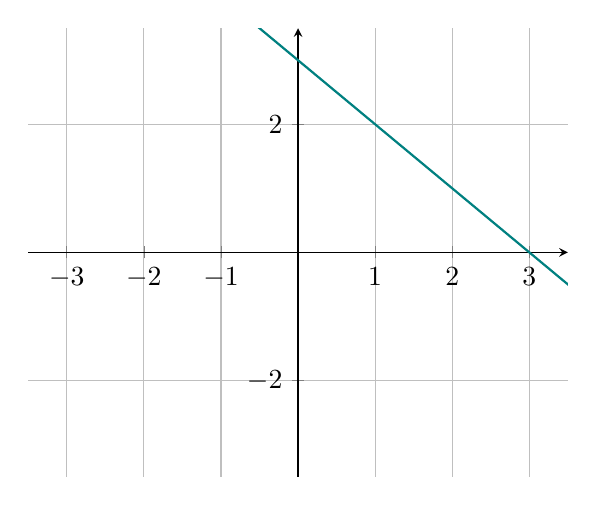
\begin{tikzpicture}
	\begin{axis}[axis lines = middle, grid,xmin = -3.5, xmax = 3.5, ymin = -3.5,ymax = 3.5]
		\addplot[color = teal, thick] {-x+3};
	\end{axis}
\end{tikzpicture}
}
\resizebox{0.45\textwidth}{0.45\textwidth}{
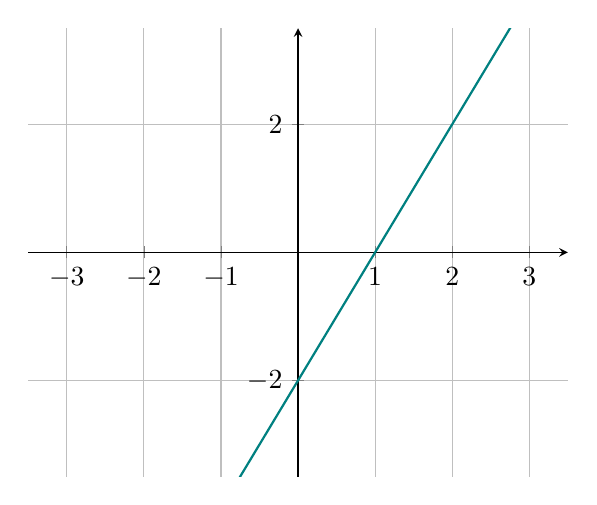
\begin{tikzpicture}
	\begin{axis}[axis lines = middle, grid,xmin = -3.5, xmax = 3.5, ymin = -3.5,ymax = 3.5]
		\addplot[color = teal, thick] {2*x-2};
	\end{axis}
\end{tikzpicture}
}
\resizebox{0.45\textwidth}{0.45\textwidth}{
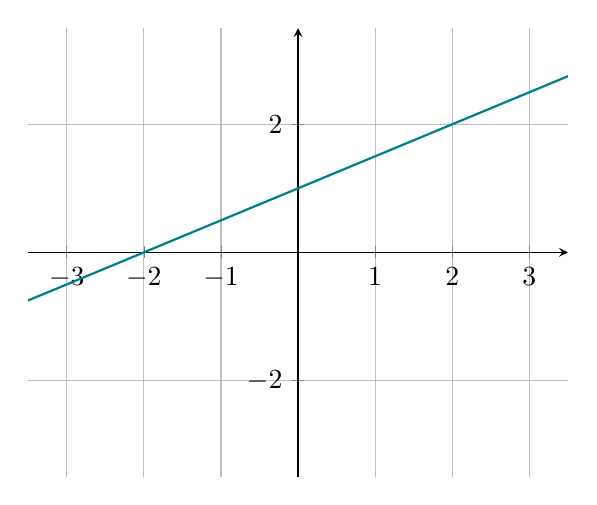
\begin{tikzpicture}
	\begin{axis}[axis lines = middle, grid,xmin = -3.5, xmax = 3.5, ymin = -3.5,ymax = 3.5]
		\addplot[color = teal, thick] {0.5*x+1};
	\end{axis}
\end{tikzpicture}
}
\resizebox{0.45\textwidth}{0.45\textwidth}{
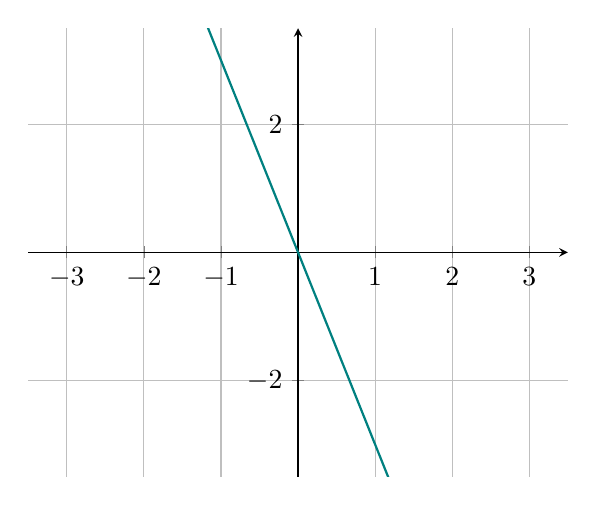
\begin{tikzpicture}
	\begin{axis}[axis lines = middle, grid,xmin = -3.5, xmax = 3.5, ymin = -3.5,ymax = 3.5]
		\addplot[color = teal, thick] {-3*x};
	\end{axis}
\end{tikzpicture}
}
\end{center}

\subsection*{Opgave 11}
En linje $l$ er givet ved parameterfremstillingen
	\begin{align*}
		l: \begin{pmatrix}
			x \\ y
		\end{pmatrix}
		= 
		\begin{pmatrix}
			2 \\ 3
		\end{pmatrix} + 
		t
		\begin{pmatrix}
			-4 \\ 6
		\end{pmatrix}
	\end{align*}

\begin{enumerate}[label=\roman*)]
	\item Bestem den værdi for $t$, hvor $l$ skærer $x$-aksen.
	\item Bestem det punkt, hvor $l$ skærer $y$-aksen. 
	\item Bestem det punkt, hvor $l$ skærer linjen med ligningen $y = 12$.
\end{enumerate}

\subsection*{Opgave 12}
En linje $l$ er givet ved parameterfremstillingen
\begin{align*}
	l: \begin{pmatrix}
		x \\ y
	\end{pmatrix}
	=
	\begin{pmatrix}
		5 \\ -5
	\end{pmatrix} +
	t
	\begin{pmatrix}
		2 \\ 3
	\end{pmatrix}
\end{align*}
og en linje $m$ er givet ved ligningen
\begin{align*}
	-3(x+4) + 2(y-1) = 0
\end{align*}
\begin{enumerate}[label=\roman*)]
	\item Afgør, om $l$ og $m$ er orthogonale. 
	\item Bestem det punkt, hvor $l$ og $m$ skærer hinanden. 
\end{enumerate}

